\documentclass[10pt, conference]{IEEEtran}
\usepackage{amssymb,amsthm,amscd,bm}
\usepackage[cmex10]{amsmath}

\usepackage{listings}
\lstset{language=C++, basicstyle=\normalsize}

\usepackage{graphicx}

\usepackage[tight,footnotesize]{subfigure}

\usepackage[named]{algo}

\usepackage{url}

\usepackage{tabularx}

%\usepackage{times}
%\usepackage{expdlist}

\newcommand{\ib}[1]{\textbf{#1}}
\newcommand{\gC}{\ib{C}}
\newcommand{\gD}{\ib{D}}
\newcommand{\gF}{\ib{F}}
\newcommand{\gG}{\ib{G}}
\newcommand{\gH}{\ib{H}}
\newcommand{\gK}{\ib{K}}
\newcommand{\gR}{\ib{R}}
\newcommand{\gL}{\ib{L}}
\newcommand{\gO}{\ib{O}}
\newcommand{\gV}{\ib{V}}
\newcommand{\gRs}{\gR_s}
\newcommand{\gRx}{\gR_{\times}}
\newcommand{\gI}{\ib{I}}
\newcommand{\gN}{\ib{N}}
\newcommand{\gP}{\ib{P}}
\newcommand{\gf}{\ib{f}}
\newcommand{\gp}{\ib{p}}
\newcommand{\gs}{\ib{s}}
\newcommand{\ga}{\ib{a}}
\newcommand{\gb}{\ib{b}}
\newcommand{\gc}{\ib{c}}
\newcommand{\gd}{\ib{d}}

\newcommand{\inrhd}{i_{\nrhd}}
\newcommand{\inlhd}{i_{\nlhd}}
\newcommand{\isim}{i_{\sim}}

\newcommand{\cR}{\mathcal{R}}
\newcommand{\cRs}{\cR_s}
\newcommand{\cRx}{\cR_{\times}}

\newcommand{\nT}{\mathbb{T}}
\newcommand{\Nat}{\mathbb{N}}

\newcommand{\gFs}{\gF^*}
\newcommand{\gFu}{\gF^{\cup}}

\newcommand{\executes}{\textit{executes}}
\newcommand{\pure}{\textit{pure}}
\newcommand{\params}{\textit{params}}
\newcommand{\func}{\textit{func}}
\newcommand{\adj}{\textit{adj}}
\newcommand{\any}{\textit{any}}
\newcommand{\isPrim}{\textit{isPrimitive}}
\newcommand{\isSol}{\textit{isSolution}}
\newcommand{\isPartSol}{\textit{isPartSolution}}
\newcommand{\fixed}{\textit{fixed}}
\newcommand{\children}{\textit{children}}
\newcommand{\type}{\textit{type}}
\newcommand{\merge}{\textit{merge}}
\newcommand{\adjacent}{\textit{adjacent}}
\newcommand{\parents}{\textit{parents}}
\newcommand{\loc}{\textit{loc}}
\newcommand{\offset}{\textit{offset}}
\newcommand{\vtable}{\textit{vtable}}

\newcommand{\positive}{\textit{positive}}
\newcommand{\sequence}{\textit{sequence}}
\newcommand{\nlhd}{\ntriangleleft}
\newcommand{\nrhd}{\ntriangleright}

\newcommand{\bs}{$\blacksquare$}

\newtheorem{statement}{Statement}
\newtheorem{rulez}{Rule}
\newtheorem{lemma}{Lemma}
\newtheorem{theorem}{Theorem}
\newtheorem{cmr}{Consistency maintenance rule}

\newcommand{\compact}{}
\newcommand{\listingsize}{\normalsize}

%\pagestyle{empty}

\pagestyle{plain}

\begin{document}

\title{Reconstruction of Class Hierarchies for Decompilation of C++ Programs}

\author{
    \IEEEauthorblockN{
        A. Fokin\IEEEauthorrefmark{1},
        K. Troshina\IEEEauthorrefmark{2} and
        A. Chernov\IEEEauthorrefmark{3}
    }
    \IEEEauthorblockA{
        \IEEEauthorrefmark{1}
        Computational Math. and Cybernetics Dept.\\
        Moscow State University,\\
        Leninskie Gory, Moscow, Russia\\
        Email: apfokin@gmail.com
    }
    \IEEEauthorblockA{
        \IEEEauthorrefmark{2}
        Institute for System Programming\\
        Russian Academy of Sciences,\\
        25, Alexander Solzhenitsyn st., Moscow, Russia\\
        Email: katerina@ispras.ru
    }
    \IEEEauthorblockA{
        \IEEEauthorrefmark{3}
        Computational Math. and Cybernetics Dept.\\
        Moscow State University,\\
        Leninskie Gory, Moscow, Russia\\
        Email: cher@unicorn.cmc.msu.ru
    }
}

\maketitle
\thispagestyle{plain}

\begin{abstract}
This paper presents a method for automatic reconstruction of
polymorphic class hierarchies from the assembly code obtained by
compiling a C++ program.
If the program is compiled with run-time type information (RTTI),
class hierarchy is reconstructed via analysis of RTTI structures.

In case RTTI structures are missing in the assembly, a technique
based on the analysis of virtual function tables, constructors and
destructors is used.
First, the inheritance relation on a set of virtual function tables
induced by inheritance relation on a set of classes is reconstructed.
Then additional analysis of constructors and destructors is used to
reconstruct inheritance relation on a set of classes.

A tool for automatic reconstruction of polymorphic class hierarchies,
which implements the described technique, is presented.
This tool is implemented as a plugin for IDA Pro Interactive Disassembler.
Experimental study of the tool is provided.
\end{abstract}

\begin{IEEEkeywords}
decompilation; reverse engineering; C++; class hierarchy reconstruction;

\end{IEEEkeywords}





\section{Introduction}
Decompilation from low-level machine languages to high-level
languages (especially C) has gained fair amount of attention
recently. Decompilers have been improving in quality and range
of accepted low-level programs. The C programming language
was chosen a target language for decompilers essentially
because it is simple enough, yet powerful and widely used.

Typical applications of decompilation are binary auditing
and malware analysis \cite{emmerik07}. A lot of modern software
is written in C++ or C/C++ mix, and the use of
C++ in malware is also increasing \cite{sabanal07}.
However, decompilation of C++
programs into C results in undesirable artifacts, including
non-decompiled assembly fragments in place of C++ exception
handling operators, or a mess of C types instead of C++
inheritance hierarchy. Therefore recovering of C++ specific
language features is important for quality decompilation.
This work is a step on this way.

In this work we present a method for reconstruction of
hierarchies of polymorphic classes from the assembly code obtained
by compiling a C++ program.
We presume
that no modifications of the assembly code were performed
after compilation (such as assembly-level obfuscation).
The problem of obtaining the assembly code from an executable file
lies outside of the scope of this work.

If the program was compiled with RTTI (run-time type information)
enabled, hierarchy of polymorphic classes is
reconstructed
exactly as it was in the source C++ program. Multiple and
virtual inheritance\footnote{Virtual
inheritance and inheritance utilizing virtual functions are
two distinct C++ concepts. Virtual inheritance is closely related
to multiple inheritance and deals with cases of inheriting the
same class more than once. Virtual inheritance does not necessarily
define a polymorphic class hierarchy \cite{stroustrup97}.}
are handled correctly. As run-time type
information structures store class names, class names are also
recovered.

If the program was compiled without RTTI,
an induced inheritance relation on
a set of vtables (virtual function tables) is considered.
This relation is reconstructed via analysis of vtables and vtable accesses.
Multiple inheritance is handled via additional analysis of
constructors and destructors.
Virtual inheritance is not handled.
%In this case we also presume that virtual inheritance is not used.
%Multiple inheritance is partially handled by gathering
%information on vtables.

Presented methods were implemented as a plugin for IDA Pro 
interactive disassembler \cite{ida} and have been tested on a variety
of open-source C++ software.
For implementation we considered C++ ABI
(application binary interface) of Microsoft Visual Studio
compiler on Windows platform and C++ ABI
of GNU C++ compiler on Windows. We used MSVC 9.1 and g++ 4.3
for experimental study, but the tool also works for
other versions of these compilers provided they use the same C++ ABI.

This paper is organized as follows. Section
\ref{sectionRelatedWork} discusses related work.
Class hierarchy reconstruction via analysis of RTTI structures
is presented in Section \ref{sectionRTTIAnalysis}.
Section \ref{sectionNoRTTIAnalysis} presents the methods for class
hierarchy reconstruction without RTTI structures.
The experimental results are discussed in Section \ref{sectionExperiments}.
Our conclusions and directions for future work are
presented in the last section.




\quad

\section{Related work}
\label{sectionRelatedWork}
% !!!
There are a lot of important works on decompilation.
In our opinion,
the following works are the closest to the topic of this paper.

Skochinsky \cite{skochinsky06} has given a detailed description
of RTTI structures used by MSVC
along with implementation details of some of the C++ concepts,
such as constructors, destructors, and exception handling.
He has presented a tool for automatic analysis of RTTI structures
and has successfully used it for polymorphic class hierarchy
reconstruction. The tool has been implemented as a script for IDA Pro
interactive disassembler.

Van Emmerik et al. \cite{emmerik04} have described
the experience gained from applying
a native executable decompiler
assisted by a commercial disassembler and hand editing
to a real-world Windows-based application.
Authors were able to recover almost all original class names
and a complete class hierarchy via analysis of RTTI structures.

However, RTTI structures may not be present in the assembly, and in
such cases it is impossible to use the methods proposed in the
above-mentioned works.

Sabanal and Yason \cite{sabanal07} along with RTTI-based approach
have proposed a technique based on the analysis of vtables and
constructors that can be applied even when RTTI structures are
not present in the assembly.
Vtable analysis is used for polymorphic class identification
and class relationship inference is done via constructor analysis.
Authors have also presented several examples of successful class
hierarchy reconstruction.
However, several cases, in which presented techniques may fail, are
not considered.
These cases include \lstinline{operator new} overloading,
constructor inlining and elimination of vtable references in
constructors due to optimizations.
Presented techniques also heavily rely on the usage of
Microsoft-specific \textbf{\_\_thiscall} calling convention.

In the paper we present a new approach to polymorphic class
hierarchy reconstruction based on the analysis of vtables,
vtable accesses, constructors and destructors.




\quad

\section{Analysis of RTTI structures}
\label{sectionRTTIAnalysis}

\subsection{Run-time type information in C++}
Run-time type information in C++ is used for
implementing the following operators \cite{stroustrup97}.
\begin{itemize}\compact
\item The \lstinline{dynamic_cast<>} operator.
    This operator performs type conversions with run-time checking.
    Normally it is used to
    convert a pointer to a base class to a pointer to a
    derived class, or to convert a lvalue referring
    to a base class to a reference to a derived class.
    A program can thereby use a class hierarchy safely.
\item \lstinline{typeid} operator. This operator provides a program 
    with the ability to retrieve the actual type of an object referred 
    to by a pointer or a reference.
\end{itemize}

The \lstinline{typeid} operator can be applied to non-polymorphic types.
In this case it is evaluated at compile time.
On the contrary, the \lstinline{dynamic_cast<>} operator works
with polymorphic types only, and results in undefined behavior
in case the program was compiled without RTTI.

The layout of RTTI structures used for implementing
\lstinline{typeid} and \lstinline{dynamic_cast<>} operators
is defined by the ABI (application binary interface) that is used by the C++ compiler.
The layout varies from compiler to compiler and from platform to platform.
For example, MSVC uses an undocumented format,
which, however, has been successfully reverse-engineered
and can be looked up in source code of Wine or, for example,
in \cite{skochinsky06}.
The ABI used by GCC can be looked up in \cite{gccabi}.
The layout of RTTI structures used in GCC is defined in
the \lstinline{<cxxabi.h>} header file, which is supplied with the compiler.

In this paper we presume that the format of RTTI structures
used by the compiler is known and can be parsed.



\quad

\subsection{Class hierarchy reconstruction}
In case RTTI structures are present in the assembly,
the process of class hierarchy reconstruction can be split
into the following steps.
\begin{enumerate}\compact
\item Locate RTTI structures.
\item Parse RTTI structures.
\item Use obtained information to reconstruct a polymorphic class hierarchy.
\end{enumerate}

%The layout of RTTI structures in assembly is determined
%by the ABI used.
As there are quite few different RTTI layouts,
it is practical to repeat the above steps several times,
once for each layout,
and then choose the most plausible variant manually.

In certain cases it is possible to determine the compiler used (and therefore, the ABI).
For example, it can be determined by analyzing the standard library
the program uses. If the standard library is linked dynamically,
the compiler can easily be determined given the shared library file.
If the standard library is linked statically, then
its vendor can be determined via function signature comparison. % ref to sigsearch?

Given the layout and position of RTTI structures in the assembly,
parsing them imposes no difficulties.
Full polymorphic class hierarchy
can then be reconstructed by merging all partial class hierarchies
obtained from RTTI structures.



\quad

\subsection{Locating the RTTI structures}
\label{chapterLocatingRTTI}
In all ABIs known to the moment pointer to the RTTI structure
of a class always precedes the corresponding vtable.
Therefore, the problem of finding the RTTI structures can be reduced
to a problem of locating vtables.
For each vtable the following statements hold.
\begin{itemize}\compact
\item Vtable is an array of pointers to functions.
\item Only the first element of the vtable
    is referenced from the program code~--- its address
    is used in constructors and a destructor of the corresponding class.
\end{itemize}

Therefore, vtables can be located by scanning the data segment and
checking each location in it.
\begin{itemize}\compact
\item If current location is referenced from code segment and
    its value is a pointer to a function, then it is marked as
    a start of vtable. Otherwise, scan is continued.
\item Other elements of vtable must be unreferenced
    pointers to functions, so finding the size of vtable is
    straightforward. Vtable ends with the first 
    location that is either referenced from program code,
    or is not a pointer to a function.
\end{itemize}





\quad

\section{Absence of RTTI structures}
\label{sectionNoRTTIAnalysis}

Run-time type information in C++ programs
is frequently misused \cite{stroustrup93},
and some modern applications written in C++ refrain from using it.
In case RTTI is not used, vtables are still generated for each polymorphic class.
However, uniqueness of vtables for each class
is not guaranteed, i.e. the same vtable
may be shared by several different classes.
For example, if some class \lstinline{B} inheriting from class \lstinline{A}
does not override any of the virtual functions of class \lstinline{A}, then classes \lstinline{A}
and \lstinline{B} can share the same vtable. This is impossible if RTTI
is used, since RTTI structure is accessed through vtable pointer field,
and class \lstinline{A} and class \lstinline{B} are distinct classes and their corresponding
RTTI structures differ.

We can presume that induced inheritance relation on a set of vtables is single,
i.e. each vtable inherits from at most one parent vtable,
as we do not handle virtual inheritance. Therefore, vtable inheritance hierarchy
consists of several inheritance trees.

A set of all vtables
can be built using the method described in chapter \ref{chapterLocatingRTTI}.
For two vtables $B$ and $D$, we say that vtable $B$ is a direct base of vtable $D$ if
one of the classes corresponding to vtable $B$ is a direct base of one of
the classes corresponding to vtable $D$.
In this case we also say that vtable $D$ inherits directly from vtable $B$,
and that vtable $D$ is a direct child of vtable $B$.
Simple inheritance for vtables can then be defined as a transitive
closure of direct inheritance. The fact that vtable $D$ inherits
from vtable $B$ is denoted as $D \rhd B$ and is also referred to as
``$B$ is a base of $D$'' and ``$D$ is a child of $B$''.

Note that $\rhd$ is a relation that defines a strict partial order on
a set of all vtables. Also the following relations are used:
\begin{itemize}\compact
\item vtable $B$ does not inherit from vtable $D$, denoted as $B \nrhd D$,
\item vtable $B$ inherits from vtable $D$, or vtable $D$ inherits from vtable $B$, denoted as $B \sim D$.
\end{itemize}

Note that if both conditions $B \nlhd D$ and $B \sim D$ are satisfied,
then condition $D \rhd B$ is also satisfied, and vice-versa. In terms
of relations it means that relation $\rhd$ is an intersection
of relations $\nlhd$ and $\sim$.

Information on inheritance relation between two vtables
can be stored as a three-bit field, with each bit indicating the
presence of one of the relations $\nrhd$, $\nlhd$ and $\sim$.
These bits are referred to as $\inrhd$, $\inlhd$ and $\isim$.
For example, if for vtable pair $(D, B)$ all bits are set to zero,
then nothing is known about the inheritance relation between vtables $D$ and $B$.
If bits $\inlhd$ and $\isim$ are set, then it is known that $D \rhd B$.
If bits $\inlhd$ and $\inrhd$ are set, then it is known that vtables
$D$ and $B$ do not inherit from each other.
All three bits being set is an indication of a conflict.
A three-bit field that encodes a relation between two vtables getting into
conflict state during reconstruction can be a consequence of some of the
presumptions on the structure of the program being false. 
The details on resolving such conflicts are provided in the description
of the algorithm in chapter \ref{chapter:full_reconstruction}.

$A_i$ denotes $i$-th virtual function in a vtable $A$.
The pointer in a virtual function table may point to an \textit{adjuster thunk}
that adjusts the passed \lstinline{this} pointer and then transfers control
to the actual function body.
In case there is no adjuster thunk, zero adjustment value is presumed.
$A_i^{\adj}$ denotes \lstinline{this} adjustment value of $i$-th virtual function in vtable $A$.




\quad

\subsection{Retrieving inheritance relation}\label{chapterRetrieving}
Several simple rules are used for inheritance relation reconstruction.
Each rule is given in a form \textit{if [antecendent], then [consequent]}.
$B$ and $D$ denote two distinct vtables, and $i$ denotes some integer.

\begin{rulez}\label{stmt:first_good}\label{stmt:vtable_size}
If the size of vtable $B$ is less then the size of vtable $D$, then $B$ cannot inherit from $D$ ($B \nrhd D$).
\end{rulez}
In compliance with the C++ inheritance rules \cite{cpp03},
if there are more virtual functions in vtable $D$ than in vtable $B$,
then $D$ cannot be a base of $B$. % !!! the base of ?

\begin{rulez}\label{stmt:inherit_pure}
If virtual function $B_i$ is pure\footnote{A virtual function is pure if it has no body, and therefore cannot be called. See \cite{stroustrup97} for details.} and virtual function $D_i$ is not, then vtable $B$ cannot inherit from vtable $D$ ($B \nrhd D$).
\end{rulez}
In C++ it is impossible to override a virtual function that is not pure
with a pure one \cite{cpp03}. For pure virtual functions both GCC and MSVC 
store a pointer to stub function in a vtable.
This stub function terminates a program with appropriate error message.
It can be reliably identified via signature matching.

If it is possible to reliably determine the size of the parameters
of a virtual function (for example, if the function uses
a calling convention where callee clears the stack),
then the following rule can be used.
\begin{rulez}\label{stmt:param_size}
If sizes of the parameters of virtual functions $B_i$ and $D_i$ are different,
then neither vtable $B$ inherits from vtable $D$, nor $D$ inherits from $B$ ($B \nrhd D \wedge B \nlhd D$).
\end{rulez}
In compliance with the C++ inheritance rules \cite{cpp03},
a virtual function cannot be overridden by a function with incompatible parameters.

The fact that some function appears on the same position in
two vtables means that it was either inherited by one of
these vtables from another, or it was inherited from some common base,
or this situation was a result of optimization.

Experiments with GCC and MSVC have shown that
neither GCC nor MSVC perform pairwise function comparison during compilation
to eliminate identical functions.
However, during compilation of a single compilation unit,
MSVC eliminates identical functions with simple bodies
like \lstinline{return /* const */}.
Further experiments have shown that there is a limit on the length
of the assembly code of a function that can be eliminated this way.
A function is called \textit{primitive} if its assembly code
is shorter than this limit, i.e. it could have been generated as a result
of identical function elimination.

\begin{rulez}\label{stmt:fsets_2}
Let {\em $\gf$} be a set of all vtables having virtual function $B_i$ on $i$-th position 
with \lstinline{this} adjustment value of $B_i^{\adj}$.
Obviously, vtable $B$ lies in {\em $\gf$}.
Then the subgraph of vtable inheritance hierarchy induced\footnote{Given graph $G = (V, E)$ and a subset of vertices $U \in V$, the subgraph of $G$ induced by $U$, denoted as $G[U]$, is a graph with vertex set $U$ and edge set consisting of all the edges from $G$ connecting vertices in $U$ \cite{rosen02}.} by {\em $\gf$} is a tree.
\end{rulez}

\begin{figure}[tb!]
\hspace{0.5cm}
\begin{minipage}[b]{1cm}
{
\lstset{basicstyle=\footnotesize}
\begin{lstlisting}
class A {
public:
  virtual void f() { /* ... */ }
};
 
class B: public A {
public:
  virtual void f() { /* ... */ }
};
 
class C: public B {
public:
  virtual void f() { A::f(); }
};
 
class D {
public:
  virtual void f() { 
    ((A*)this)->A::f();
  }
};
\end{lstlisting}
}
\end{minipage}
\caption{Example program for rule \ref{stmt:fsets_2}.}
\label{listing:inheritance_example}
\end{figure}

There are several cases when this rule cannot be applied.
Consider the program on fig. \ref{listing:inheritance_example}.
Due to optimizations a pointer to function \lstinline{A::f} might have been stored
directly in the vtable of class \lstinline{D}, which is unrelated to class \lstinline{A},
without the body of the function \lstinline{D::f} being generated.
But such trickery is rare in a real code, because it gives no real
benefits while introducing the danger of invoking undefined behavior.
While a call to function \lstinline{A::f} in function \lstinline{D::f}
is a ``dangerous'' C++, a similar function call in \lstinline{C::f}
is perfectly safe.
Due to optimizations a pointer to function \lstinline{A::f}
might have been stored directly in the vtable of class \lstinline{C}.
This also breaks rule \ref{stmt:fsets_2}. 
As it is presented on fig.~\ref{fig:fset_fail}, the subgraph of
inheritance hierarchy induced by the set $\{A, C\}$ is not a tree.
This case is a fine example of \textit{code smell} \cite{fowler99} because
the approach taken only complicates the hierarchy, while the intended behavior can
be achieved by simply inheriting class \lstinline{C} directly from class \lstinline{A}.
Such cases are also rare in a real code.
We will presume that they do not occur at all.

Fig.~\ref{fig:fset} illustrates the application of rule \ref{stmt:fsets_2}.
On this figure vtables $A$, $B$ and $D$ have
the same function \lstinline{A::f} on the first position,
and therefore the subgraph of the inheritance hierarchy induced by the set $\{A, B, D\}$ is a tree.
The same is true for the set $\{B, C, E\}$ since vtables $B$, $C$ and $E$ have the same
function \lstinline{B::g} on the second position.

Some information on inheritance relation can also be gathered
using analysis of constructors and destructors.
A constructor performs the following sequence
of operations \cite{cpp03, gray94}.
\begin{enumerate}\compact
\item Calls constructors of direct base classes.
\item Calls constructors of data members.
\item Initializes vtable pointer field(s) and
    performs user-specified initialization code in the body
    of the constructor.
\end{enumerate}

Conversely, a destructor deinitializes the object
in the exact reverse order to how it was initialized.
\begin{enumerate}\compact
\item Initializes vtable pointer field(s) and
    performs user-specified destruction code in the body of the destructor.
\item Calls destructors of data members.
\item Calls destructors of direct bases.
\end{enumerate}

\begin{figure}[tb!]
\centering
  \begin{center}
    \subfigure[][]{\label{fig:fset_fail}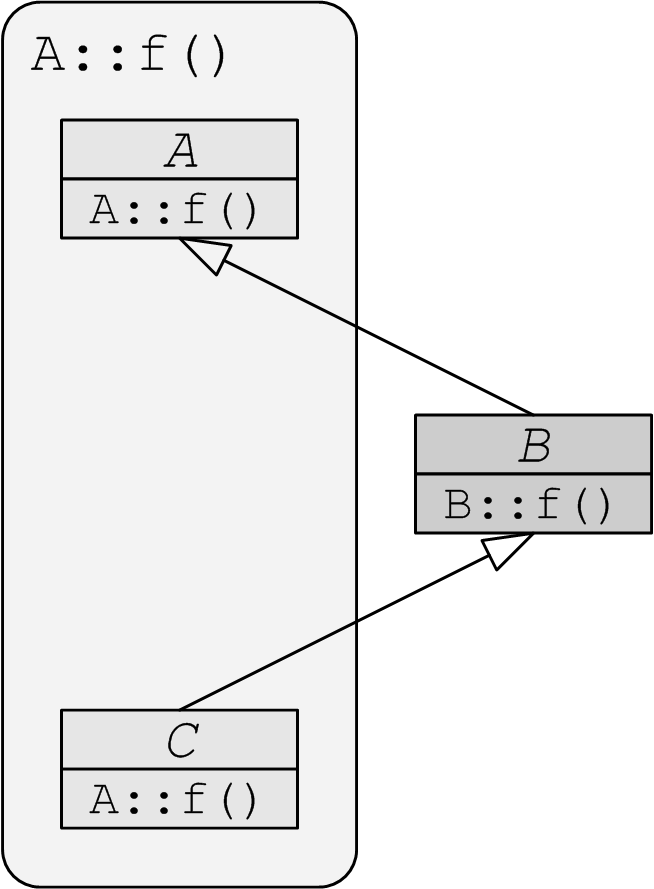
\includegraphics[scale=0.6]{images/fset_failure}}
    \subfigure[][]{\label{fig:fset}\hspace{0.3cm}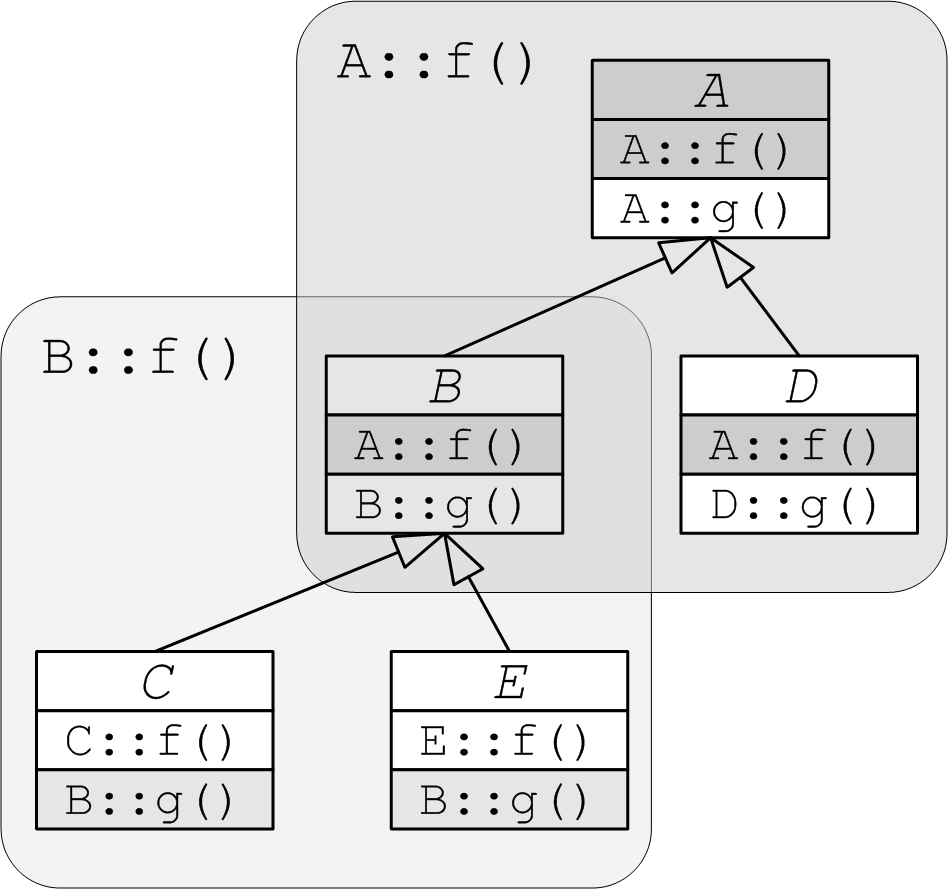
\includegraphics[scale=0.6]{images/fset}}
  \end{center}
\caption{Examples for rule~\ref{stmt:fsets_2}.}
\end{figure}

In case of a ``deep'' inheritance hierarchy,
construction and destruction of an object may require many
successive initializations of vtable pointer field(s).
Where appropriate, these assignments are optimized away by the compiler.
Experiments have shown that GCC and MSVC never optimize away
the last assignment in a virtual destructor.
That means that virtual destructor of an object always overwrites each
vtable pointer field with a pointer to the corresponding ``most-base'' vtable.
%Inheritance reconstruction method presented in this paper
%highly relies on this fact.

%Constructors and a destructor are the only functions
%that access vtable pointer field of a class.
In a call to a virtual function of some class \lstinline{D}, vtable pointer field(s) of
\lstinline{this} object can be overwritten if this function is a
virtual destructor, or as a result of a call to a constructor or a destructor of class \lstinline{D}.
The latter case is possible by using the following code:
{
\lstset{basicstyle=\listingsize}
\begin{lstlisting}
this->~D(); /* destructor */
new (this) D(/* ... */); 
    /* placement new */
\end{lstlisting}
}
\noindent or simply by executing \lstinline{delete this}. Both cases, however being rare,
have been seen in real-life production code.
% 1st one - Qt, WebKit, CMake, etc... just GoogleCode it.
% 2nd one - libmt, etc... again, use GoogleCode.
%Of course, constructor
%of some unrelated class can be called for \lstinline{this} object, but
%that would be a rather dangerous and pointless construction, so we presume
%that it does not appear in the source code.

By using interprocedural data flow analysis as it is described in \cite{aho06} for locating accesses
to vtable pointer field(s) of \lstinline{this} object inside a call to virtual function,
it is possible to find bases of a corresponding vtable using the following rule.
\begin{rulez}\label{stmt:destructors}\label{stmt:last_good}
If in a call to virtual function $D_i$ vtable pointer field corresponding to vtable $D$ 
of \lstinline{this} object is
overwritten with a pointer to vtable $B$, then $D$ inherits from $B$ ($D \rhd B$).
\end{rulez}

This rule is a direct consequence of the list of actions that must be
performed by constructors and destructors.
Moreover, if a call to destructor for \lstinline{this} object is
not followed by a call to constructor and vtable pointer field is
overwritten several times, then it is possible to infer the
inheritance relation between all the vtables referenced.
Consider the following disassembly:
{
\lstset{basicstyle=\listingsize, language=[x86masm]Assembler}
\begin{lstlisting}
; this->~D(); /* destructor */
mov dword ptr [esi], offset D::vtable
; D::~D() body goes here
mov dword ptr [esi], offset C::vtable
; C::~C() body goes here
mov dword ptr [esi], offset B::vtable
; B::~B() body goes here
\end{lstlisting}
}

Here \lstinline{this} pointer is stored in \textbf{esi} register.
Given the pattern of assignments to vtable pointer field, it can
be concluded that class \lstinline{D} inherits from class \lstinline{C},
which in turn inherits from class \lstinline{B}.

The same technique cannot be applied if a call to
destructor is followed by a call to constructor due to possibility
of some assignments to vtable pointer field being optimized away.
{
\lstset{basicstyle=\listingsize, language=[x86masm]Assembler}
\begin{lstlisting}
; this->~D(); /* destructor */
; D::~D() body was empty
mov dword ptr [esi], offset C::vtable
; C::~C() body goes here
; B::~B() body was empty
 
; new (this) D();
mov dword ptr [esi], offset B::vtable
; B::B() body goes here
; C::C() body was empty
mov dword ptr [esi], offset D::vtable
; D::D() body goes here
\end{lstlisting}
}

However, such cases can easily be detected because the last assignment
in a constructor always references the vtable being analyzed
(vtable for class \lstinline{D} in this case).

As advised by almost every guide on object-oriented design,
most of polymorphic class hierarchies are designed for
polymorphic deletion (i.e. deletion via a pointer to base class),
and therefore use virtual destructors \cite{sutter01}.
That means that in most cases rule \ref{stmt:destructors} will produce
at least one inheritance relation~--- between the vtable being analyzed
and its corresponding ``most-base'' one.



\quad

\subsection{Formalizing the problem}\label{chapterProblem}
Rules \ref{stmt:first_good}-\ref{stmt:last_good} are applied, and all
consequents are stored as a set of restrictions on the structure of
inheritance hierarchy.

Using rule \ref{stmt:destructors}
it is possible to construct a set of all vtables
in a single inheritance tree with virtual destructors.
If virtual destructors are not used, it can
still be done using rule \ref{stmt:fsets_2}.
There are some cases where it cannot be done correctly.
These cases occur if no information on inheritance
relation between two vtables can be derived from the assembly.
For example, if a base vtable $B$ consists of only one
pure virtual function, derived vtable $D$ overrides it, and
accesses to $B$ are optimized away in constructors and destructor of a class
corresponding to $D$, 
then in the assembly there is no evidence of the fact
that vtable $D$ inherits from vtable $B$.
Such cases cannot be identified automatically.
Presented algorithm produces incorrect results for them.

The set of all vtables is divided into several disjoint sets
so that all vtables in a single set form an inheritance tree
(connected inheritance hierarchy).
Global inheritance hierarchy is reconstructed by processing these
sets one by one. Let $\gV$ be one of these sets.

Let $\gR$ be a set of all restrictions concerning vtables from $\gV$
obtained by applying rules \ref{stmt:vtable_size},
\ref{stmt:inherit_pure}, \ref{stmt:param_size}, and \ref{stmt:destructors},
i.e. a set of all restrictions that can be expressed in terms of relations
$\rhd$, $\nrhd$, and $\sim$, and $\gRs$ be a set of all restrictions
concerning vtables from $\gV$ obtained by applying rule \ref{stmt:fsets_2}.

Since some presumptions have been made on the structure of the source C++ program in
chapter \ref{chapterRetrieving}, it may be possible that all obtained restrictions cannot
be jointly satisfied. We presume that all restrictions from $\gRs$ can be jointly
satisfied. If they are not, additional manual analysis will be required.
Since restrictions from $\gR$ may not be jointly satisfiable the following problem
will be considered.
\begin{equation}\label{eq:problem}
\begin{minipage}[h]{7.5cm}
Find a set of jointly satisfiable with $\gRs$ restrictions $\gR' \subseteq \gR$ so that adding
any of the elements of $\gR \setminus \gR'$ to $\gR'$ makes it jointly unsatisfiable with $\gRs$.
Build a vtable inheritance tree $T$ with nodes from $\gV$ that satisfies all the
restrictions from $\gR'$ and $\gRs$.
\end{minipage}
\end{equation}



\quad

\subsection{Reconstructing vtable inheritance hierarchy}
\label{chapter:full_reconstruction}

Each of restrictions from $\gRs$ has the form
\textit{the subgraph of vtable inheritance hierarchy induced by {\em $\gf$} is a tree}.
Let $\gF$ be a set of all such sets $\gf$.
Then, if a tree $T$ is a solution of problem (\ref{eq:problem}),
the subgraph of $T$ induced by any of the sets $\gf \in \gF$ is a tree.

Let set $\gFs$ be a set containing:
\begin{itemize}\compact
\item all sets from $\gF$,
\item all non-empty sets obtained by intersecting several sets from $\gF$,
\item set $\gV$,
\item all sets of the form $\{B\}$, where $B \in \gV$.
\end{itemize}
Note that if all subgraphs of vtable inheritance hierarchy induced by elements of
$\gF$ are trees, then the same is also true for $\gFs$.

To construct a solution of the problem (\ref{eq:problem}) graph $\gG$ that ``encodes'' all
the restriction from $\gRs$, and only them, is built. Graph $\gG$ is constructed
by modifying graph $\gH$, which is a
Hasse diagram\footnote{A Hasse diagram is a directed graph representation of
a partially ordered set in which each element is represented by a node.
Immediate successors of each element are connected
to the corresponding node with a directed edge \cite{rosen02}.}
for relation $\subset$ (\textit{is subset of}) on set $\gFs$.

Nodes of Hasse diagram $\gH$ are considered to be sets $\gf \in \gFs$,
and are assumed to possess all traits of a set~---
for example, a node can be a subset of another node.
For each node in graph $\gH$ a set of child nodes is defined as follows:
node $\gc$ is a child of node $\gp$ if there exists an edge in graph $\gH$
connecting $\gp$ and $\gc$, and $\gc \subset \gp$.

Then graph $\gG$ is built by adding new nodes to Hasse diagram $\gH$.
For each node $\gp$ of $\gH$ a set of its child nodes is considered.
If two child nodes of $\gp$ have non-empty intersection, then these
nodes are considered \textit{connected}.
The set of child nodes of $\gp$ is then divided into connected components,
and a node is added for each connected component consisting of more than one
child as it is shown on fig.~\ref{fig:gg_tree}.

\begin{figure}[tb!]
\centering
  \begin{center}
    \subfigure[][]{\label{fig:gh_example}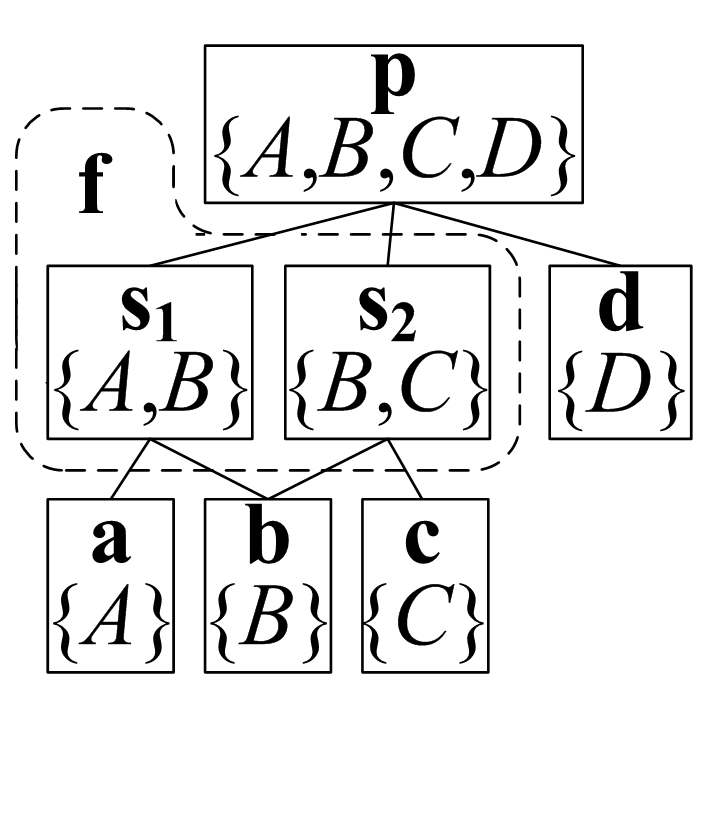
\includegraphics[scale=2.1]{images/gg_algo_class}}
    \hspace{0.1cm}
    \subfigure[][]{\label{fig:gg_example}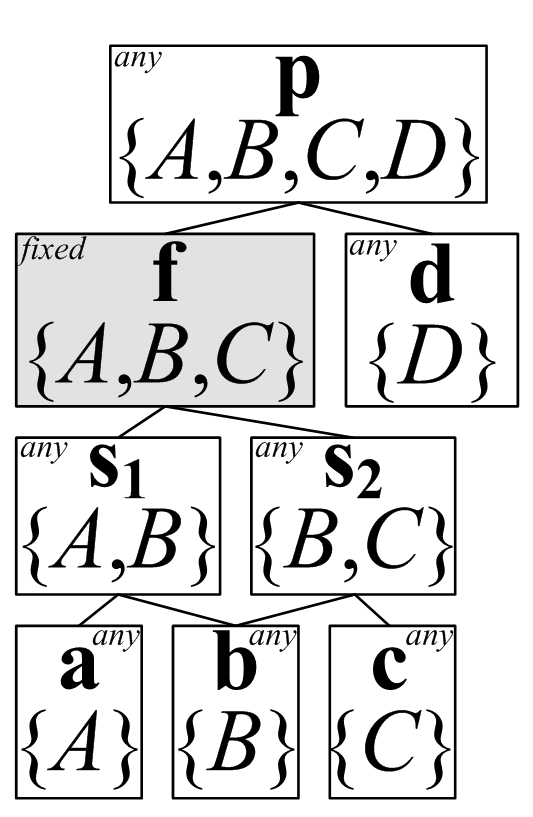
\includegraphics[scale=2.1]{images/gg_algo_class_2}}
  \end{center}
\caption{Example of graphs $\gH$ and $\gG$.}
\label{fig:gg_tree}
\end{figure}

Example of Hasse diagram $\gH$ is presented on fig.~\ref{fig:gh_example}. Child nodes
$\gs_1$ and $\gs_2$ of node $\gp$ form a connected component and therefore for these
nodes a new node $\gf$ is added, as it is shown on fig.~\ref{fig:gg_example}.
Vtable set of this node is the union of all nodes in its corresponding connected
component. Note that the resulting graph $\gG$ is also a Hasse diagram.

All newly added nodes are marked as \fixed and all the rest are marked as \any.
The meaning behind these names is as follows.
\begin{itemize}\compact
\item Children of \any-nodes do not intersect. Therefore, if induced inheritance trees
    have been built for each child of a given \any-node, then induced inheritance
    tree for this \any-node can be constructed by connecting these trees with edges~---
    total $n - 1$ edges, where $n$ is the number of children of this \any-node.
\item Children of \fixed-nodes intersect. Therefore, induced inheritance trees of the children
    of a \fixed-node fully determine the structure of the induced inheritance tree of
    this \fixed-node (i.e. its induced inheritance tree is \textit{fixed}).
\end{itemize}

For the graph $\gG$ the following statement holds.
\begin{statement}\label{theorem:evil}
If there exists a tree satisfying all the restrictions from {\em $\gRs$},
then such a tree can be constructed by building induced inheritance trees for
\any-nodes of graph {\em $\gG$} as it was described above. It will satisfy all
the restrictions from {\em $\gRs$}, regardless of how the edges to be added were
chosen at each \any-node.
\end{statement}
The proof is quite complicated, so it is not provided here.
The important idea behind this statement is that the graph $\gG$ ``encodes''
all the restrictions from $\gRs$, and only them.
Solution of the problem (\ref{eq:problem}) is built using this graph.

First, it is checked whether there are no cycles of \any-nodes in $\gG$.
It can be proven that if such cycle exists, then the problem (\ref{eq:problem})
has no solution. In this case additional manual analysis is required.

Each node of $\gG$ containing only one vtable is defined as a \textit{leaf} node
for this vtable. For each node $\gf$ and for each vtable $A$ the shortest
path from $\gf$ to the leaf node for $A$ that does not ascend into \fixed-nodes is found.
The second node in this path, which is adjacent to $\gf$, indicates a
\textit{direction} from $\gf$ to $A$, and is denoted as $\gD^{\gf}_A$. In case
such path does not exist, $\gD^{\gf}_A$ is considered to be the closest
\fixed-parent of $\gf$.

Consider an example on fig.~\ref{fig:gg_example}. Here $\gD^{\gp}_A = \gf$,
because $\ga$ is a leaf node for vtable $A$, and the shortest path from $\gp$
to $\ga$ is $(\gp, \gf, \gs_1, \ga)$. On the other hand, $\gD^{\ga}_D = \gf$,
because there exists no path from $\ga$ to $\gd$ that does not ascend into
\fixed-nodes. Therefore, $\gD^{\ga}_D$ is the closest \fixed-parent of $\ga$.

To reconstruct the resulting vtable inheritance tree $T$, for each two vtables
$B$ and $D$ a three-bit field $\gI_{(B, D)}$ containing the information
on inheritance relation between vtables $B$ and $D$ is iteratively constructed. 
Also, for
each two child nodes $\gs_1$ and $\gs_2$ of each \any-node $\gp$ of graph $\gG$,
reconstruction algorithm iteratively builds the following structures.

$\gN^{\gp}_{(\gs_1, \gs_2)}$~--- a set of all virtual tables that must be inherited
by the root vtable $R$ of inheritance tree induced by $\gs_1$ ($T[\gs_1]$)
in case one of $R$'s bases lies in $\gs_2$.

$\gP^{\gp}_{(\gs_1, \gs_2)}$~--- a set of all virtual tables that must not be inherited
by the root $R$ of $T[\gs_1]$ in case one of $R$'s bases lies in $\gs_2$.

$\gI^{\gp}_{(\gs_1, \gs_2)}$~--- three-bit field containing information on inheritance
relation between $T[\gs_1]$ and $T[\gs_2]$.
For example, if bit $\inrhd$ is set in $\gI^{\gp}_{(\gs_1, \gs_2)}$, then no base of the
root of $T[\gs_1]$ lies in $\gs_2$.

$\gRx$~--- a set of all restrictions from restriction set $\gR$ that cannot be satisfied jointly with
already processed restrictions.

\begin{figure}[tb!]
\small
\begin{minipage}[b]{0.47\textwidth}
\begin{algorithm}{ProcessRestriction}{
    \label{alg:process_restriction}
    \qinput{Vtables $B$ and $D$ and a relation $\alpha \in \{\nrhd, \sim\}$ between them.}
}
\textbf{set} bit $i_{\alpha}$ in $\gI_{(B, D)}$ \\
\textbf{let} $\ga = \text{leaf node for $B$}$ \\
\qwhile $\ga \ne \{D\}$ \qdo \\
    \textbf{let} $\gb = \gD^{\ga}_D$ and $\gc = \gD^{\gb}_D$ \\
    \qif $\gb$ is an \any-node and both $\ga$ and $\gc$ are children of $\gb$ \qthen \\
        \qif $\alpha = \: \sim$ \qthen \\
            \textbf{add} $D$ to $\gN^{\gb}_{(\ga, \gc)}$ \\
            \textbf{add} $B$ to $\gN^{\gb}_{(\gc, \ga)}$ \\
            \textbf{set} bit $\isim$ in $\gI^{\gb}_{(\gc, \ga)}$ \\
        \qelse \qcom{If we got here then $\alpha = \: \nrhd$} \\
            \textbf{add} $D$ to $\gP^{\gb}_{(\ga, \gc)}$
        \qfi \\
    \qelseif $\gb$ is a \fixed-child of $\ga$ \\
        \textbf{break}
    \qfi \\
    $\ga \gets \gb$
\qelihw
\end{algorithm}
\end{minipage}
\end{figure}

The outline of the algorithm is as follows.
\begin{enumerate}\compact
\renewcommand{\theenumii}{.\arabic{enumii}}
\renewcommand{\theenumiii}{.\arabic{enumiii}}
\renewcommand{\labelenumii}{\theenumi\theenumii)}
\renewcommand{\labelenumiii}{\theenumi\theenumii\theenumiii)}
\item All sets $\gN^{*}_{(*, *)}$, $\gP^{*}_{(*, *)}$,
    $\gI^{*}_{(*, *)}$ and $\gI_{(*, *)}$ are set to empty.
\item \label{item:next_restriction}
    A new restriction $r$ from restriction set $\gR$ is selected and placed into restriction processing queue.
    If it is a restriction of the form $D \rhd B$, then it is first decomposed into
    $D \sim B$ and $D \nlhd B$. If there are no unprocessed restrictions in $\gR$, then
    execution is continued from step \ref{item:build_child_trees}.
    \begin{enumerate}\compact
    \item \label{item:spreading}
        If restriction processing queue is empty, then execution continues from step
        \ref{item:check_tree_existence}.
        If restriction processing queue is not empty, then a single restriction is picked from
        it and processed using algorithm \ref{alg:process_restriction}.
        \begin{enumerate}\compact
        \item Algorithm \ref{alg:process_restriction} modifies sets $\gI_{(*, *)}$,
            $\gN^{*}_{(*, *)}$, $\gP^{*}_{(*, *)}$ and $\gI^{*}_{(*, *)}$.
            For modified sets consistency maintenance rules are applied.
            These rules are described in the end of the chapter.
        \item If modification results in a conflict in one of the sets $\gI_{(*, *)}$ or
            $\gI^{*}_{(*, *)}$, then $r$ is added to $\gRx$, all sets are returned to their state 
            prior to processing
            of restriction $r$ and execution is continued from step \ref{item:next_restriction}.
        \item Consistency maintenance rules add new restrictions to the restriction processing
            queue. Execution continues from step \ref{item:spreading}.
        \end{enumerate}
    \item \label{item:check_tree_existence}
        It is checked whether for each \any-node $\gp$ there exists
        a tree with vertices from a set of its children satisfying $\gI^{\gp}_{(*, *)}$.
        If such tree does not exist, then $r$ is added to $\gRx$ and
        all sets are returned to their state prior to processing of $r$.
        Execution continues from step \ref{item:next_restriction}.
    \end{enumerate}
\item \label{item:build_child_trees}
    For each \any-node $\gp$ a rooted tree $T_{\gp}$ with vertices from a set
    of its children satisfying all $\gI^{\gp}_{(*, *)}$ is constructed.
    Existence of such tree has been checked on step \ref{item:check_tree_existence}.
\item \label{item:build_sol}
    For each \any-node $\gp$ an induced inheritance tree $T[\gp]$ is
    constructed. Nodes are processed in from-child-to-parent order, so that
    the tree for node $\gp$ is constructed only when trees for all children
    of $\gp$ have already been constructed.
    Trees $T[\gp]$ and $T_{\gp}$ can be seen as directed graphs
    with edges directed towards the root of the tree.
    For each directed edge $(\gs_1, \gs_2)$ of the tree $T_{\gp}$
    an edge connecting the root vtable $R$ of $T[\gs_1]$ and a vtable
    from $\gs_2$ is added to $T[\gp]$ so that all nodes from
    $\gN^{\gp}_{(\gs_1, \gs_2)}$ are reachable from $R$ via directed
    edge walk, and all nodes from $\gP^{\gp}_{(\gs_1, \gs_2)}$ are not.
    Existence of such edge is ensured by consistency maintenance rules.
\end{enumerate}

Consistency maintenance rules mentioned in the description of the algorithm
propagate changes made to sets $\gN^{*}_{(*, *)}$, $\gP^{*}_{(*, *)}$ and
$\gI^{*}_{(*, *)}$ so that a single change in one of the sets may result
in many consequent cascade changes in other sets. Some examples
of consistency maintenance rules follow.

%\begin{enumerate}\compact
%\item \label{item:intersect_rule}
\begin{cmr}
If for some node {\em $\ga$} and its children {\em $\gs_1$} and {\em $\gs_2$},
set {\em $\gN^{\gp}_{(\gs_1, \gs_2)} \cap \gP^{\gp}_{(\gs_1, \gs_2)}$}
is not empty, then bit $\inrhd$ is set in {\em $\gI^{\gp}_{(\gs_1, \gs_2)}$}.
\end{cmr}
In other words, the only way to satisfy both conditions
$B \in \gN^{\gp}_{(\gs_1, \gs_2)}$ (vtable $B$ must be inherited by the root vtable $R$
of $T[\gs_1]$ in case one of $R$'s bases lies in $\gs_2$) and
$B \in \gN^{\gp}_{(\gs_1, \gs_2)}$ (vtable $B$ must \textbf{not} be inherited by the root
of $T[\gs_1]$ in case one of its bases lies in $\gs_2$) is for no
base of the root of $T[\gs_1]$ to lie in $\gs_2$.

\begin{cmr}
If for some node {\em $\gp$} and its children {\em $\gs_1$} and {\em $\gs_2$},
condition {\em $\gs_2 \subseteq \gP^{\gp}_{(\gs_1, \gs_2)}$} is satisfied, then
bit $\inrhd$ is set in {\em $\gI^{\gp}_{(\gs_1, \gs_2)}$}.
\end{cmr}
In other words, the only way to satisfy a condition that
all vtables from $\gs_2$ must not be inherited by the root of
$T[\gs_1]$ in case one of its bases lies in $\gs_2$ is
for none of its bases to lie in $\gs_2$.

The set of all vtables
has been divided into several disjoint sets, so that all vtables in a single set
form a connected inheritance hierarchy.
The described algorithm is applied for each of these sets
thus
reconstructing the full vtable inheritance hierarchy.



\quad

\subsection{Reconstructing polymorphic class hierarchy}\label{chapterMultiple}
Correspondence between vtables and actual classes is reconstructed
via constructor and destructor analysis. The information obtained is then used for
multiple inheritance inference.

Interprocedural data flow analysis is used to detect
code sites, where one or more memory locations each one differing
from each other by a constant offset, are overwritten with
pointers to vtables.
These code sites are referred to as \textit{vtable access sites}.
Every such site is associated with
a set of pairs (\positive\:\offset, \vtable\:\sequence).
Vtables are stored in a sequence in which their addresses
were written at the corresponding offset to the memory location
being tracked.

On this step full information on inheritance relation
between vtables is available and therefore
each vtable access site with one of the vtable sequences containing
more than one element can be classified as being either
a constructor or a destructor. 

Consider the program on fig. \ref{listing:chained_example} for
for two vtables $B$ and $D$, $D$ inheriting $B$.
Associated set of pairs is $\{(0, (B, D)), (8, C)\}$.
Since vtable $D$ inherits from vtable $B$, this vtable access site is 
classified as a constructor.

\begin{figure}[tb!]
\hspace{0.5cm}
\begin{minipage}[b]{1cm}
{
\lstset{basicstyle=\listingsize, language=[x86masm]Assembler}
\begin{lstlisting}
 mov ecx, esi
 call sub_40BBB0
 mov dword ptr [esi], offset D::vtable
 ; ...
 mov dword ptr [esi+8], offset C::vtable
 ; ...
 
sub_40BBB0 proc near
 ; this looks like a constructor of
 ; a base class
 push esi
 mov esi, ecx
 mov dword ptr [esi], offset B::vtable
 ; ...
\end{lstlisting}
}
\end{minipage}
\caption{Example program for classifying a vtable access site as either a constructor or a destructor.}
\label{listing:chained_example}
\end{figure}

In case each sequence in the associated set consists of
only one element, this method cannot be used. Instead, the
following rules are used.
\begin{enumerate}\compact
%\item As it was pointed out in chapter \ref{chapterRetrieving}, virtual
%destructors always overwrite the vtable pointer field with a
%pointer to the ``most-base'' vtable. They are are also referenced
%from the vtable and therefore can be easily detected.
%
% The idea behind this one - if site is referenced from vtable and accessed vtable differs from it, then we have 2 vtables %).
%
\item Constructor and destructor calls, if not inlined, are nested:
constructor calls constructors for base classes, etc.
Therefore, once a vtable access site has been classified as either
a constructor or a destructor, vtable access sites to the same memory
location in all nested calls are classified as having the same type.
\item Constructors and destructor for ``most-base'' classes
overwrite vtable pointer field only once, and therefore
cannot be easily differentiated if not nested into some other
constructor or destructor. That's why in this case they are
associated with a corresponding set of (\offset, \vtable\:\sequence) pairs
and classified as being unidentified.
\item If all these rules fail to identify the vtable access
site, then the case is reported to the user. % zero reports so far
\end{enumerate}

After completing vtable access site analysis, for each site
classified as being either a constructor or unidentified, the
corresponding set of (\offset, \vtable\:\sequence) pairs
is transformed. Last vtable is picked from each sequence
thus producing a set of (\offset, \vtable) pairs. In
accordance to the actions performed in constructor, each
such pair identifies a unique class, with vtables being
the virtual tables belonging to this class and offset values
being offsets to instances of the corresponding base classes.

Generally speaking, the fact that vtable belongs to a class does not
necessarily mean that this class has inherited it.
The class at hand may just include as a field some other class
that owns this vtable.
However, polymorphic classes are normally included by pointer.
Besides, inclusion by value differs from inclusion by inheritance
only if virtual destructors are involved (in this case a pointer to
the same virtual destructor must be stored in all vtables of a class).
That's why by default we presume that all vtables belonging to
a class have been generated as a result of inheritance.
%Cases of class's vtables having different virtual destructors
%are reported to the user. zero reports so far

Constructors and destructors for ``most-base'' abstract classes
may not have been generated by the compiler. That's why for each
root vtable that contains pure virtual functions
a class containing it at offset 0 is constructed.

\begin{figure}[tb!]
\centering
  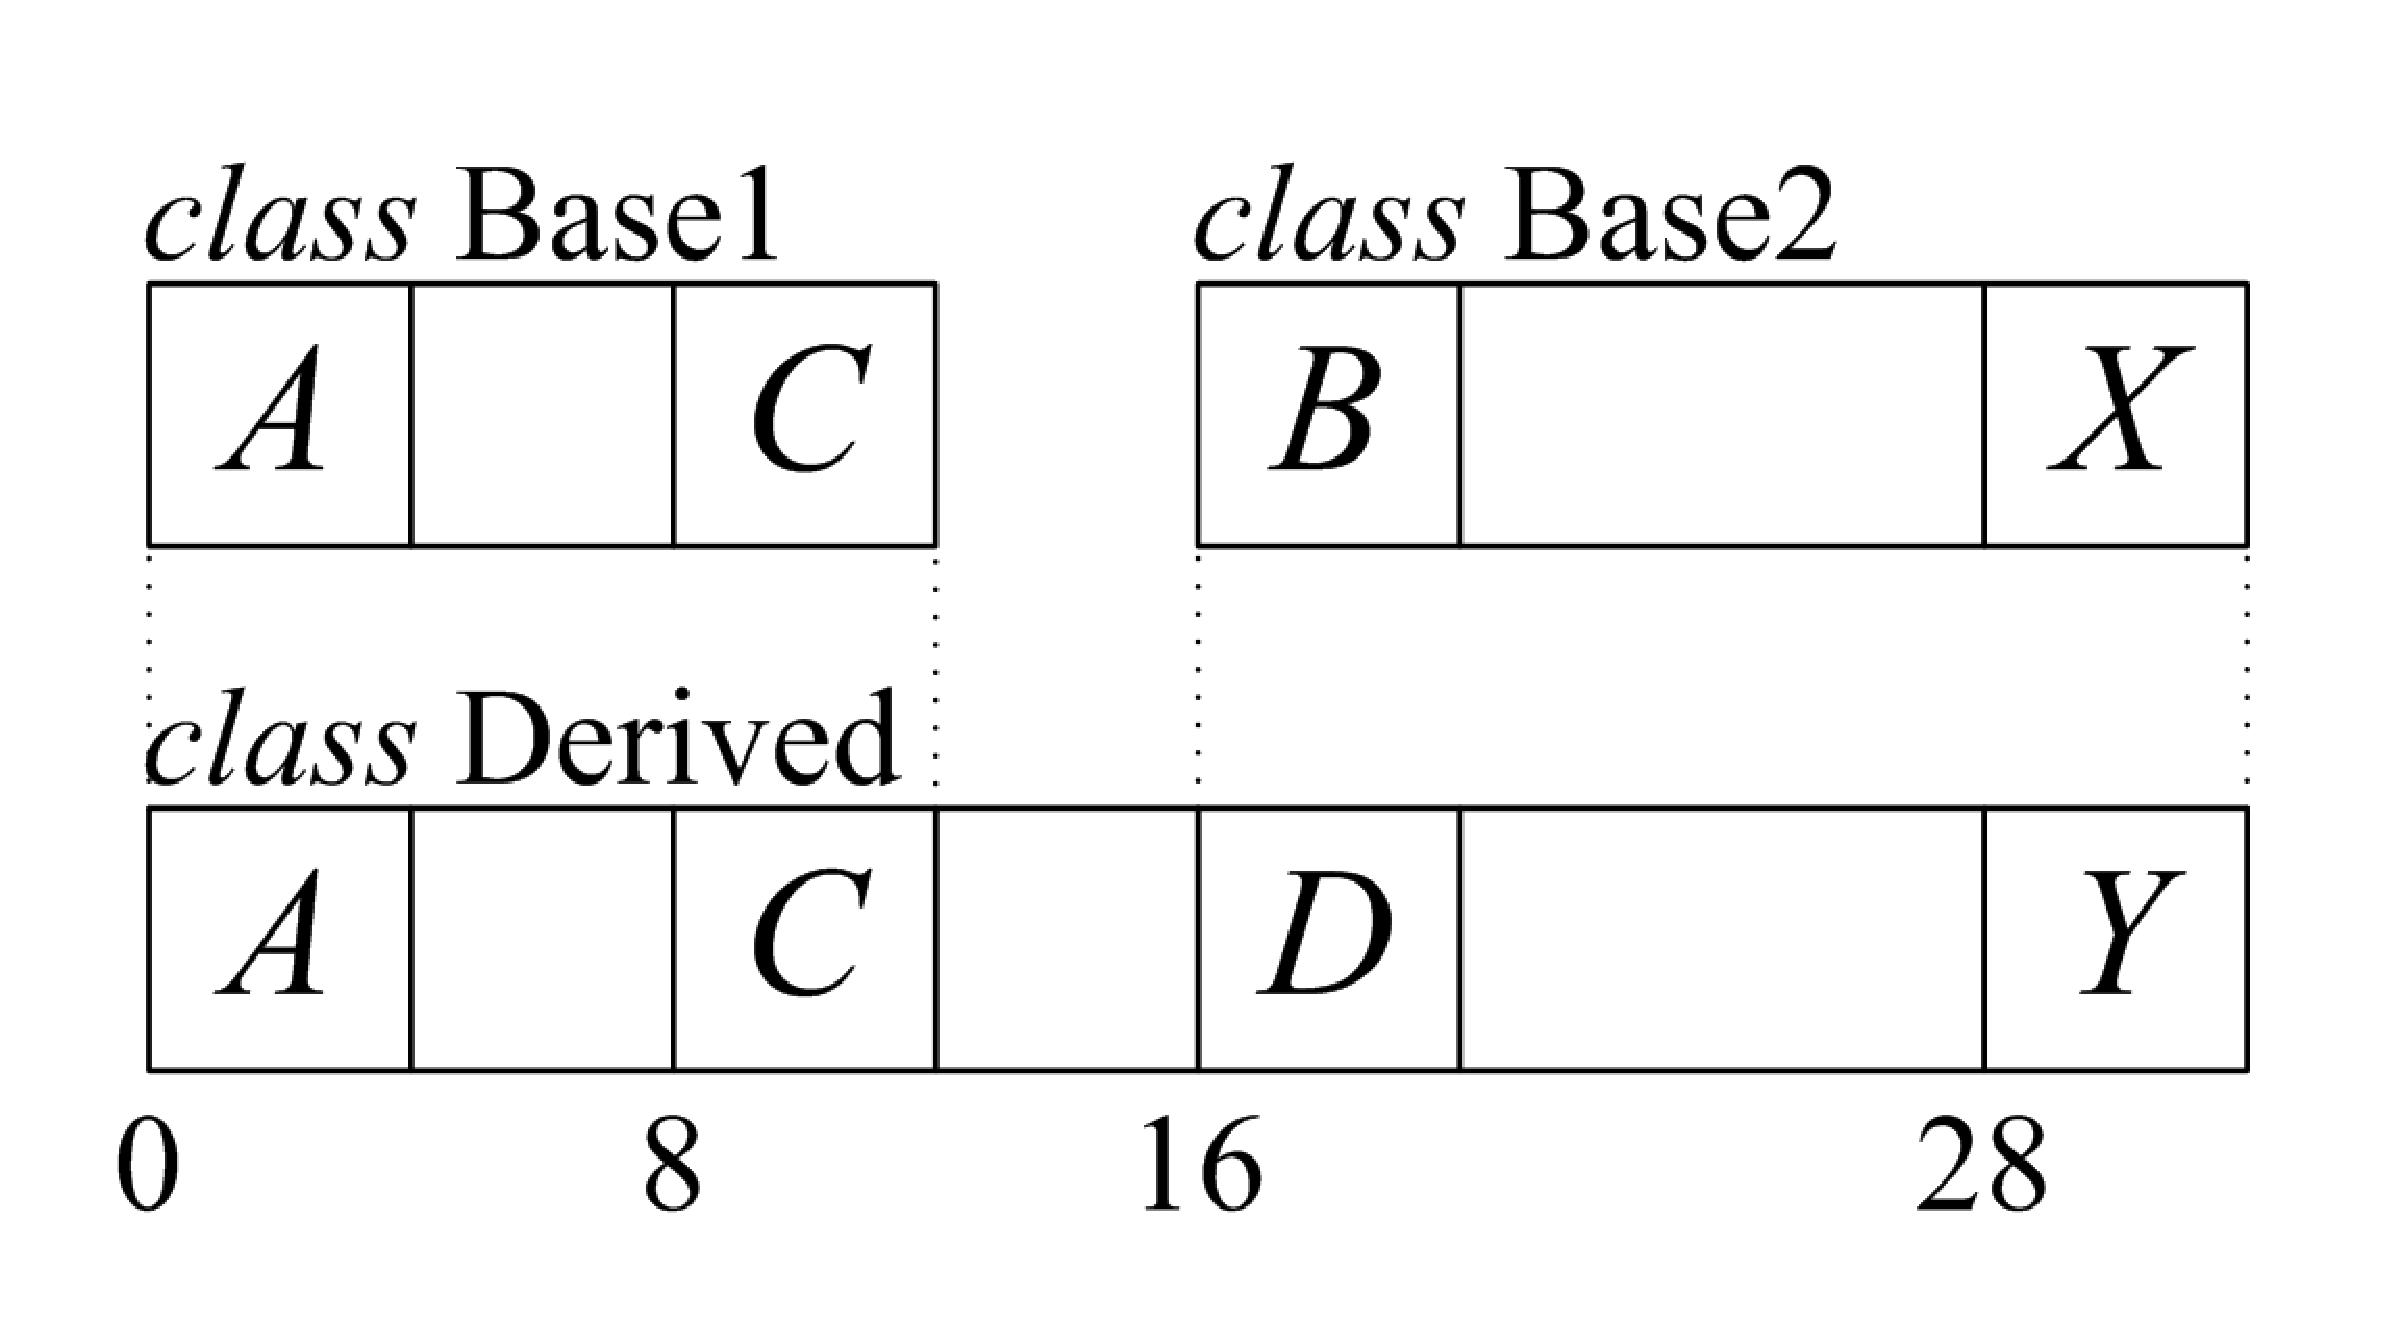
\includegraphics[scale=1.80]{images/multiple}
\caption{Example of base class matching.}
\label{fig:multiple}
\end{figure}

After a set of classes is constructed, inheritance relation inference
is performed.
For each class a set of possible direct base classes is constructed.
Class \lstinline{Base} can be a direct base of class \lstinline{Derived}
if it can be ``placed'' inside class \lstinline{Base} so that overlapping
vtables are either equal or connected by direct inheritance. Example
is given on fig.~\ref{fig:multiple}. Here vtable $B$ is a direct
base of $D$, and vtable $X$ is a direct base of $Y$. Pair sets associated
with classes are $\{(0, A), (8, C), (16, D), (28, Y)\}$ for
class \lstinline{Derived}, $\{(0, A), (8, C)\}$ for class \lstinline{Base1}
and $\{(0, B), (12, X)\}$ for class \lstinline{Base2}. Placement of
both classes \lstinline{Base1} and \lstinline{Base2} inside
class \lstinline{Derived} satisfies the mentioned conditions,
and therefore these classes can be direct bases of class \lstinline{Derived}.

Normally, there exists only one way to ``cover'' a class with
base classes. In case there are several coverings, then the one with
the largest number of vtables being equal to the vtables of the
class at hand is selected. If there are several such coverings,
the case is reported to the user. % zero reports so far

Inheritance relation inference finishes class hierarchy reconstruction.
As a result, for each class in a program the following is reconstructed.
\begin{enumerate}\compact
\item Direct base classes with offsets to the corresponding instances.
\item Vtables and offsets to these vtables.
\item Constructors and destructors for non-``most-base'' classes.
\end{enumerate}



\quad

\subsection{Complexity analysis}

Algorithm for vtable search described in chapter \ref{chapterLocatingRTTI} depends
linearly on the size of program data segment.
The complexity of data flow analysis algorithm used in chapters \ref{chapterRetrieving}
and \ref{chapterMultiple} depends linearly on the size of the program being analyzed.

%Then all the rules from chapter \ref{chapterRetrieving}
%can be applied in $O(n^2)$ operations.
The most computationally difficult part of the inheritance reconstruction
process is the one described in chapter \ref{chapter:full_reconstruction}.
Compared to it, computational complexity and memory requirements of
multiple inheritance reconstruction algorithm described in
chapter \ref{chapterMultiple} can be neglected.

We presume that the maximal size of vtable is a constant that can be neglected in
the computational complexity estimations.
Let $n$ be a number of vtables found in the program being analyzed.
The number of different functions in vtables is $O(n)$. Therefore,
the size of the set $\gF$ is also $O(n)$. The size of the set $\gFs$ depends
exponentially on $n$, because it includes the intersection closure of $\gF$.
Let $N$ be the size of the set $\gFs$.

It can be proven that the number of nodes in graph $\gG$ is
$O(N)$, the total size of all sets $\gN^{*}_{(*, *)}$ and $\gP^{*}_{(*, *)}$ and all fields
$\gI^{*}_{(*, *)}$ is $O(nN)$, and the total size of all fields $\gI_{(*, *)}$
is $O(n^2)$. Therefore, the memory requirements of the presented algorithm is
$O(nN)$.

Set $\gFs$ and graph $\gG$ are constructed in $O(nN^2)$ operations.
The total computational complexity of all other steps of the algorithm
is $O(n^3N)$.

\begin{figure}[tb!]
\centering
  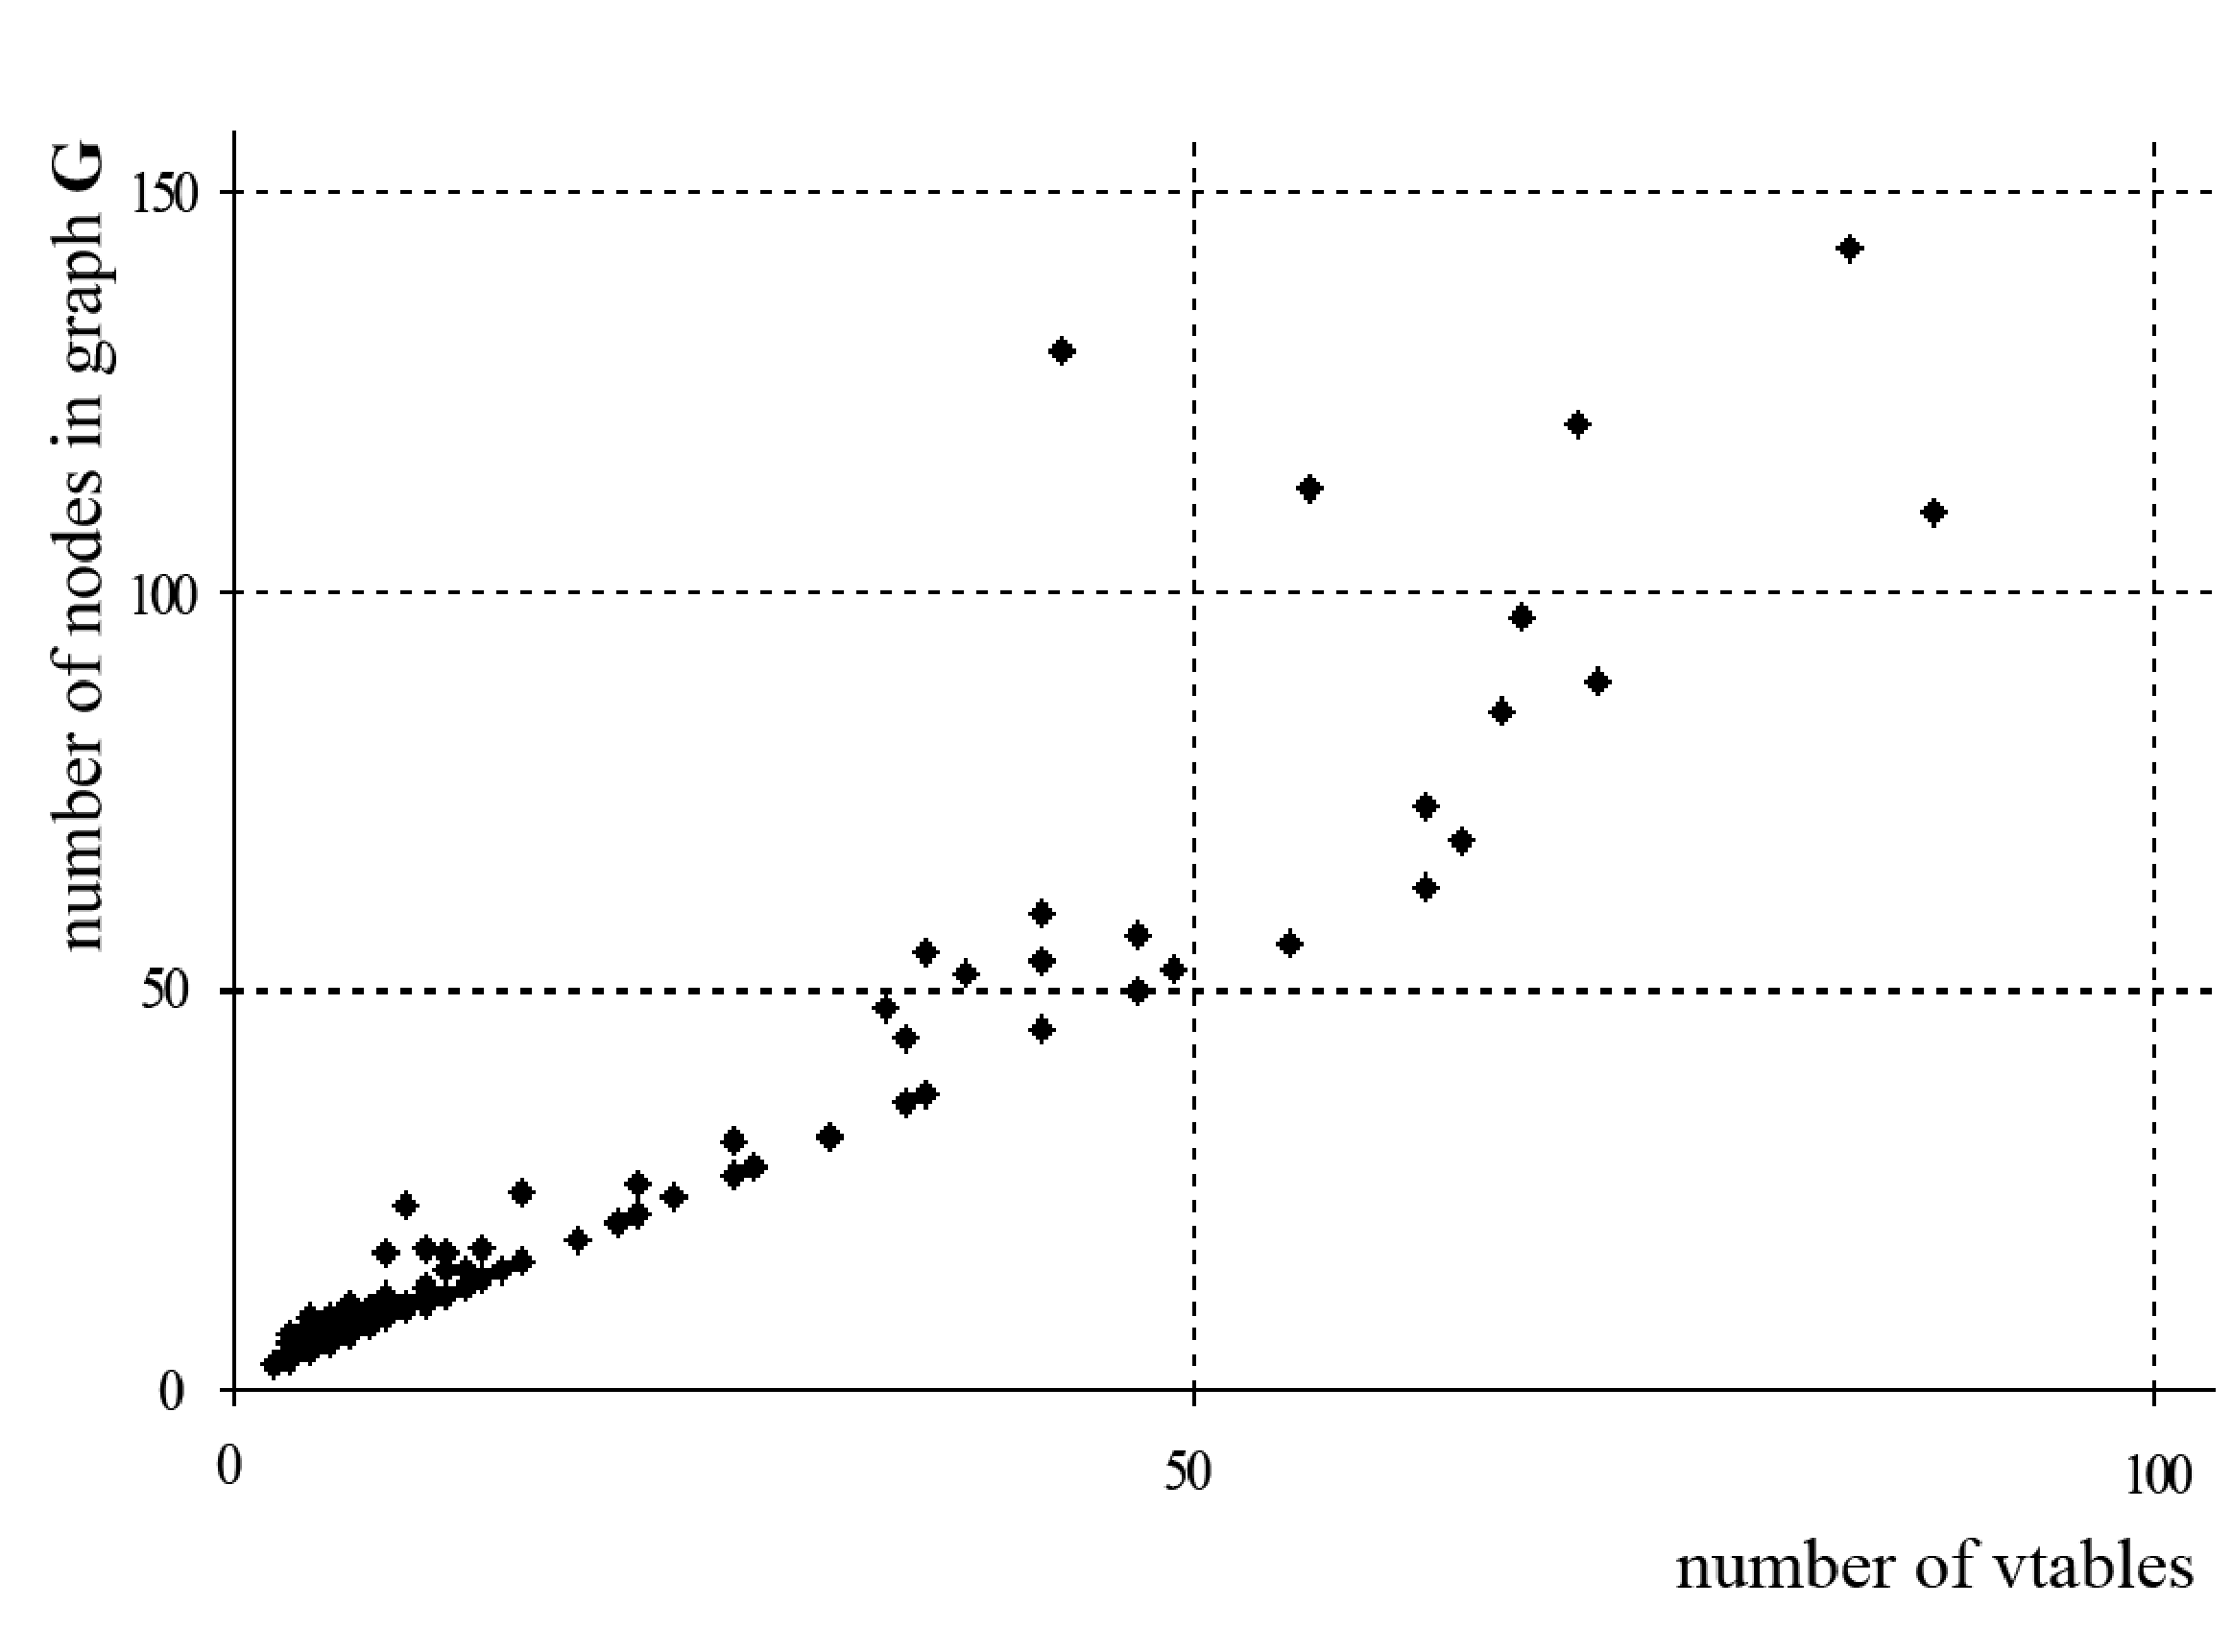
\includegraphics[scale=0.22]{images/fstar_size}
\caption{Experimental results on the size of set $\gFs$ depending on the number of vtables.}
\label{fig:fstar_size}
\end{figure}


Exponential computational complexity may seem impractical.
However, experiments have shown that this is not the case and in
practice the size of the set $\gFs$ is not that big.
For connected class hierarchies of size less than 100 classes statistics have
been gathered by applying the algorithm to several open-source
projects, including doxygen (source code documentation generator tool),
Notepad++ (text editor), Shareaza (peer-to-peer file sharing client),
mkvmerge (application for merging multimedia streams into a Matroska file),
VirtualDub (video capture and processing utility), and others.
Results are presented on fig.~\ref{fig:fstar_size}. As it can
be seen, in most cases the size of the set $\gFs$ does not exceed $2n$.
Therefore, the estimation of computational complexity of the
algorithm is $O(n^4)$.
More experimental data on running times of the algorithm is
given in section \ref{sectionExperiments}.

In most cases class hierarchies consisting of over 100 classes are 
hierarchies with a single ``universal base class'' like
\lstinline{QObject} in Qt library, 
\lstinline{CObject} in MFC library
and \lstinline{wxObject} in wxWidgets library.
Such hierarchies use RTTI in one
form or another, and therefore the application of
the algorithm presented in section \ref{sectionNoRTTIAnalysis} is not
needed for them. 
Besides, hierarchies of over 100 classes often become overly
complex and hard to maintain, forcing programmers to use
\lstinline{dynamic_cast<>} operator to deal with
unforeseen problems. The usage of this operator requires compilation with RTTI. 





\quad

\section{Implementation and experimental results}\label{sectionExperiments}
Presented methods have been implemented completely in C++ as a plugin
for IDA Pro interactive disassembler. The plugin is available for
download at web page \url{http://www.decompilation.info}.
The plugin consists of several weakly bound modules, which can be reused
in other contexts. These modules are as follows.
\begin{enumerate}\compact
\item C++ wrapper for the functionality offered by IDA Pro.
\item Implementation of data flow analysis algorithm.
\item Implementation of class hierarchy reconstruction algorithm based on the analysis of RTTI structures.
\item Implementation of class hierarchy reconstruction algorithm described in
    chapters \ref{chapter:full_reconstruction} and \ref{chapterMultiple}.
\end{enumerate}

The plugin has been tested on a variety of open-source software written in C++.
The process used is as follows.
\begin{enumerate}\compact
\item The program is compiled with optimizations and RTTI enabled.
\item RTTI-aware class hierarchy reconstruction algorithm is used to reconstruct
    the polymorphic class hierarchy exactly as it is in the source files.
\item The program is compiled with optimizations and debug information but without RTTI.
\item Class hierarchy reconstruction algorithm that does not use RTTI structures
    is applied.
\item Debug information is used to restore the correspondence between vtables and
    polymorphic classes.
\item Results of the two class hierarchy reconstruction algorithms are compared.
\end{enumerate}

\begin{figure}[htb!]
\begin{tabular}{| l | r | r | r |}
\hline
Application &         doxygen & Shareaza & Notepad++ \\
\hline
Running time &          7.9s  &   18.9s  & 0.7s \\
\hline
Vtables found &         444   &   1381   &  98 \\
\hline
Non-vtables &           6.5\% &   18.3\% & 3.0\% \\ % 253
\hline
Vtable mismatches &     8.6\% &    4.1\% & 4.0\% \\
\hline
Classes found &         401   &   1108   &  95 \\
\hline
Class mismatches &      9.7\% &    5.7\% & 4.2\% \\
\hline
\end{tabular}
\caption{Test results.}
\label{fig:tests}
\end{figure}

Plugin was tested on a Core2Duo CPU at 2.8Ghz.
Some of the test results are presented on fig. \ref{fig:tests}. 
\begin{itemize}\compact
\item ``Non-vtable'' refers to a vtable that actually is a mere array of pointers.
    Debug information is used to check for this.
\item ``Vtable mismatch'' refers to a vtable with reconstructed parent vtable differing
    from the real one.
    Note that this is not necessarily an error since in many cases small disturbances
    in hierarchy structure do not change the semantics of the program. For example, if all
    classes in a hierarchy have only two virtual functions, no data members, trivial
    constructors and destructors, and always override only the first function,
    then inheritance order does not matter because the code produced
    will be the same.
\item ``Classes found'' refers to the number of polymorphic classes found
    during reconstruction.
\item ``Class mismatch'' refers to a class with associated vtables or parents
    reconstructed differently from the real ones. Again, in many cases this
    is not an error due to the same reasons as with mismatched vtables.
\end{itemize}

In all tests non-vtables found during reconstruction have formed an inheritance
tree consisting of a single node. 
Furthermore, the access pattern for these vtables was different. 
Normally a vtable is accessed by writing its address into memory. 
In case of an access to non-vtable, its address is often written into a register.
Therefore, even though there were a lot of non-vtables in some test cases, 
these non-vtable were easily identified.

Study of vtable and class mismatch cases has shown that the results obtained
do not contradict the information used in the analysis. In some of the considered
mismatch cases the mismatch was caused by violation of one of presumptions
the algorithm relies on (such as usage of virtual inheritance).
In most cases the mismatched vtable (class) just happened to be
several levels up or down the hierarchy, preserving pairwise inheritance
relations to the most of the other vtables (classes) in the hierarchy.

There were also a small number of cases when the tool has failed to reconstruct
the inheritance relation between several classes, outputting them as unrelated.
These cases are the ones pointed out in the beginning of chapter \ref{chapterProblem}.

To further decrease the
mismatch rates, additional analysis is required, such as dynamic analysis
and deeper analysis of the actions performed in constructors and destructors.





\quad

\section{Conclusion and further work}
A method for automatic reconstruction of polymorphic class hierarchies
from assembly code obtained by compiling a C++ program is presented.
If the source C++ program is compiled with run-time type information enabled,
then the class hierarchy is reconstructed exactly in the same form as it
was in the source code.

If RTTI is not compiled into the assembly, reconstruction
method is based on the analysis of virtual function tables, constructors and destructors.
First, inheritance relation on a set of virtual tables is reconstructed using
the analysis of virtual function tables and virtual function table accesses.
Then additional analysis of constructors and destructors is used to restore
classes and relations between them. Multiple inheritance is handled
correctly.

Proposed methods were implemented as a plugin for IDA Pro interactive disassembler,
which is currently available for download.
The plugin has been tested on a variety of open-source software written in C++
showing low mismatch rates.

Directions of future work include deeper analysis of constructors
and destructors to further increase the accuracy of class hierarchy
reconstruction, as well as reconstruction of exception handling
blocks and other C++ features.
The main goal is to develop several techniques that could be implemented
as a set of tools for reconstructing low-level programs into C++ 
programming language.


\quad


\bibliographystyle{IEEEtran}
\bibliography{article}

\end{document}

% Local variables:
%  compile-command: "dopdf.bat"
% End:

